% !TEX program = pdflatex
\documentclass[journal]{IEEEtran}

% ============================================================
%  Packages
% ============================================================
\usepackage[T1]{fontenc}
\usepackage{amsmath,amssymb,amsfonts}
\usepackage{algorithmic}
\usepackage{algorithm}
\usepackage{array}
\usepackage{booktabs}
\usepackage{multirow}
\usepackage{cite}
\usepackage{graphicx}
\usepackage{textcomp}
\usepackage{xcolor}
\usepackage{url}
\usepackage{hyperref}
\usepackage{tikz}
\usepackage{tabularx}
\usepackage{threeparttable}
\usepackage{makecell}
\usepackage{enumitem}
\usepackage{balance}
\usepackage{subcaption}
\usepackage{pdflscape}

\usetikzlibrary{positioning, arrows.meta, shapes.geometric, fit, backgrounds, calc, decorations.pathreplacing}

\hypersetup{
  colorlinks=true,
  linkcolor=black,
  citecolor=black,
  urlcolor=blue
}

\setlist{nosep}

% Custom commands
\newcommand{\ie}{\textit{i.e.}}
\newcommand{\eg}{\textit{e.g.}}
\newcommand{\etal}{\textit{et al.}}

\begin{document}

% ============================================================
%  Title
% ============================================================
\title{AMTTP: A Four-Layer Architecture for Deterministic Compliance Enforcement in Institutional DeFi}

\author{
  \IEEEauthorblockN{Odeyemi Olusegun Israel}
  \IEEEauthorblockA{Independent Researcher\\
  Derby, United Kingdom\\
  Email: segettii@gmail.com}
}

\maketitle

% ============================================================
%  Abstract
% ============================================================
\begin{abstract}
Decentralized finance has transformed the global capital markets significantly enough to provide a platform for automatic transactions, remove a need for an intermediary, and reduce the time it takes to settle transactions. However, the level of institutional involvement in DeFi remains very low. The lack of institutional participation can be attributed to the lack of an enforceable compliance mechanism at the protocol level; that is once a transaction is confirmed as having been completed on the blockchain, it can't be undone or disputed in any meaningful way. The existing compliance mechanisms are primarily retrospective, meaning that they generate alerts after a transaction has occurred instead of preventing illicit transfers in advance. Regulated financial institutions that transact in cryptocurrency bear the ultimate financial risk and regulatory burden. The UK FCA has made it very clear through CP25/41 that there now are specific regulatory expectations regarding the existence of adequate pre-settlement controls~\cite{fca2025}.

We introduce AMTTP Version~4.0, which has been designed to have a four-layer architecture explicitly intended to support deterministic compliance enforcement in DeFi institutions. Layer~I provides SDKs, REST APIs, and web applications intended for programmatic and human interaction with AMTTP; Layer~II provides a compliance orchestration layer that combines (i)~machine learning risk scoring (ii)~graph analysis (iii)~sanctions screening, and (iv)~policy adjudication into a single deterministic decision-making matrix; Layer~III consists of an offline training pipeline with a Composite Teacher that uses an Autoencoder-Enhanced XGBoost ($w = 0.4$), seven FATF AML Mode Patterns ($w = 0.3$), and graph structural properties ($w = 0.3$) in order to produce pseudo-labels (SLPs) for the Student pipeline across 2,640,000 transactions; and finally, Layer~IV supports the physical infrastructure for AMTTP deployment, which consists of 18 smart contracts on Ethereum Sepolia, 17 containerised microservices, and a Database Persistence Tier (MongoDB, Redis, Memgraph, IPFS). The Infrastructure Security features multi-oracle threshold signatures, replay protection \& zkNAF a zero-knowledge proof framework that allows for privacy preserving verification of KYC credentials, risk ranges \& non-membership from sanctions. In addition, TLS Encryption, Rate Limiting, Cloudflare Tunnel integration \& the UI Integrity Service provide an additional layer of protection at the infrastructure level. This paper aims to demonstrate that deterministic compliance can be integrated into Decentralized Finance (DeFi) at an architectural level. In order to support this assertion, the complete specifications will be made available as infrastructure as code.\footnote{Source code: \url{https://github.com/segetii/fintech}}
\end{abstract}

\begin{IEEEkeywords}
DeFi Compliance, AML, Oracle Architecture, Transaction Enforcement, Institutional Finance, Smart Contracts, Zero-Knowledge Proofs
\end{IEEEkeywords}

% ============================================================
%  I. INTRODUCTION
% ============================================================
\section{Introduction}

Decentralised finance has upended much of what was settled about financial infrastructure. Transactions execute on blockchain networks without brokers, clearing houses, or custodian, which significantly reduces transaction costs, and settling them in seconds instead of days or weeks; therefore also eliminating entire classes of intermediaries. The efficiency dividend is apparent, however the compliance deficit is very much real, especially for institutional investors who must adhere to stringent regulatory obligations such as pension schemes, sovereign wealth funds and asset management companies.

Regulating bodies have labelled this ``The DeFi Compliance Paradox''. By monitoring suspicious transactions through traditional finance platforms, the regulator can stop the transfer in-flight, review it for any illicit activities, and reverse the transfer if there's a potential illegal market participant prior to the transaction settling. This is impossible with permissionless blockchains, where finality occurs in seconds. Upon finality, the transaction becomes unalterable---it's a done deal. No matter how sophisticated the monitoring or analytics tools are, they cannot reverse the action once it has been executed, and therefore institutions that participate in transactions without pre-settlement controls run the risk of being sanctioned by regulatory bodies; suffering reputational damage; and/or becoming inadvertently involved with illicit capital.

The growth of regulation is becoming evident. The UK will have a comprehensive crypto regulatory framework, with AML and counter-terrorism financing programs starting in October of 2027~\cite{fca2025}. The rest of the world is a patchwork of different concepts, different expectations, and capital requirements that, for most treasurers at institutions, are too burdensome.

In general, DeFi AML tools that are currently on the market today can be described as being mostly reactive in their operation. Chainalysis and Elliptic provide off-chain analytics to identify suspicious patterns and generate alerts; these are definitely useful, but none of these tool systems can prevent a high-risk transaction from completing it. Academically, numerous studies have greatly increased the accuracy of detection mechanisms (\eg, GraphSAGE) but still generate outputs that have no means of stopping the transfer. This paper explains how to use an application programming interface (API) called Anti-Money Laundering Transaction Trust Protocol (AMTTP) to include the expectations associated with conducting transactions, such as anti-money laundering. The design combines machine learning risk assessment with graph-based and deterministic references and tools using smart contracts, which will be distributed in four layers of a full stack solution. The use of a zero knowledge configuration will allow for privacy compliant auditing, relative to General Data Protection Regulation (GDPR) regulated transactions~\cite{groth2016}; therefore the AMTTP is an actual working application, contained as a full applicable production version with an operational dashboard for monitoring compliance in real time.

% ============================================================
%  II. RELATED WORK
% ============================================================
\section{Related Work}

There has been a substantial increase over the last 5 years in scholarship regarding DeFi Compliance due primarily to the growing gap between traditional AML/CFT regimes and modern decentralised protocols. Early academic works on the risk of blockchain applied somewhat broad or even vague definitions of ``risk,'' whereas recent scholarship has become much more focused on privacy-preserving regulation, on-chain real-time enforcement, and the particular issues faced by institutional participants in DeFi~\cite{joseph2025}.

Commercial anti-money laundering platforms (such as Chainalysis, Elliptic, etc.)\ utilise a centralised monitoring approach to perform retrospective analysis on each transaction. These platforms are able to produce graph-based traces, use heuristic pattern matching and generate alerts before a transaction occurs; however, none of these platforms are able to stop a transaction from going through on a permissionless blockchain, where finality occurs almost instantly (\ie, in seconds)~\cite{memgraph2024}.

From a research perspective, the techniques we have used from machine learning to improve the detection of transactions on graphs has made significant strides. Specifically, the use of GraphSAGE and other graph neural networks (GNNs) on transaction graphs is an example of how well they can identify wallet-to-wallet interactions at the wallet level. In fact, GNN methods routinely achieve over 0.90 ROC-AUC scores on standard datasets. To demonstrate how far these methods have come, since they are only being used on off-chain data, none of the existing techniques enforce any actions or changes on the blockchain ledger itself~\cite{hamilton2017}.

The authors of this article have compiled a comprehensive compilation of commercial platforms (41) and academic prototypes (28) studied between 2015--2025. They have further broken down these studies into categories based upon three domains: regulatory evolution, verifying layer compliance and lifecycle phases (preventative, real-time and investigative). Based on the findings of this paper the authors contend that the utilisation of WEB3 architectures will ultimately provide benefits for transaction graph analytics, real-time scoring, cross-chain monitoring and privacy preserving verification at levels that currently challenge centralised systems. However, the authors also identify numerous challenges related to the use of WEB3 architectures including, but not limited to: limited cross-chain coverage, minimal ability to monitor DeFi interactions, very little oversight of privacy protocols and MVC scalability---all of which will require further work before widespread adoption in production environments can take place~\cite{mao2025}.

Approaches that preserve privacy come into play as part of the dichotomy between data protection law and compliance obligations. Zero-knowledge proofs provide compliance with regulatory requirements by establishing proof of compliance with certain attributes, such as non-sanctioned status, while not disclosing the underlying data~\cite{groth2016}. Therefore, zero-knowledge proof systems, specifically Groth16 circuits, will be in alignment with the requirements of the General Data Protection Regulation (GDPR) and have significant implications for companies implementing these types of systems. For example, on the one hand, zkAML uses ZK-SNARKs to enable whitelist-based anti-money laundering (AML) activities within smart contracts while providing cryptographic assurances to regulators that the activities are compliant with regulations and are also cryptographically protected from unauthorized access to personal user information. On the other hand, verifiable credentials push this idea even further by allowing for attestation of regulatory compliance without disclosing personal and sensitive user information~\cite{alego2025}.

Moving to more proactive enforcement, new architectures using multi-agents are being an evolution in the direction of proactive enforcement. Khanvilkar \etal\ have proposed a decentralized multi-agent system that distributes regulatory rules among multiple agents using formal logic, a consensus protocol, and a zero-knowledge technique~\cite{khanvilkar2025}. The immutable nature of smart contracts is the basis of the audit trail. The reported accuracy at low latency exceeds 98\%, there are no single points of failure in the design, and it is capable of operating across jurisdictions---all of which are necessary features that cannot be optional for institutional participation.

Compliance Frameworks for Distributed Systems (ensuring consistency, immutability, and auditability) build on top of four layers: ingestion, ledger, processing, and audit. Furthermore, neighbouring structures are formed as layers from already built neighbouring sites are used to construct subsequent neighbouring sites~\cite{gade2025}. In both cases, the same layered structure has been used in human resource management through blockchain technologies and fixed-income tokenisation. The structures are designed for transparency and codified rules~\cite{madanchian2026}. They provide the foundation for the deterministic enforcement on the blockchain, but only a very small number of entities have implemented a complete AML pipeline solution that provides graph temporal analytics from end to end.

The world of decentralised finance (DeFi) is making a concerted effort to work with institutions. Mohapatra and Raut analyse how corporations can use DeFi protocols for treasury and liquidity management. They believe that using DeFi provides increased efficiency, but highlight that governance is critical in order to achieve those efficiencies~\cite{mohapatra2025}. Meanwhile, Olanrewaju emphasises the importance of securitisation of DLT (Distributed Ledger Technology) on the DeFi platform while providing detail on compliance and interoperability barriers and potential solutions through oracle networks and KYC-integrated contracts~\cite{olanrewaju2025}.

AMTTP builds upon all existing frameworks previously developed, including and similar to those described earlier; likewise, AMTTP addresses the largest void observed, which is in the area of pre-emptive (proactive) enforcement prior to settlement. In order to complete deterministic actions on-chain, off-chain analytics (ML via ensembles and the temporal graph) feed into on-chain actions through a four-layered, structured process. Various existing tools currently document and create alerts for identified items within their ecosystem; however, AMTTP will enable users to normalise disparate signals, thus enabling the user to make real-time compliance decisions of `approve', `review', `escrow' or `block'.

To provide this capability, zkNAF creates a privacy-preserving layer of attestation that bridges the reactive surveillance systems used today and that required for institutions to complete their business at an actual institutional-grade level~\cite{fca2025,fatf2023}.

In conclusion, the comprehensive body of work clearly illustrates the advancements in detection and privacy. However, when observed holistically, it is clear there is no full-stack (production-grade), protocol-enabled AML enforcement mechanism specifically designed for institutional DeFi. AMTTP will fulfil that need~\cite{sivaraju2024,ogunmola2025,campbell2026}.

% ============================================================
%  III. SYSTEM ARCHITECTURE
% ============================================================
\section{System Architecture}
\label{sec:arch}

The chart shows the protocol segmented into layers, as shown in Fig.~\ref{fig:architecture}; each layer has a specified area of coverage. From an audience perspective on enforceable on-chain actions, these boundaries for the layers are intentionally separated from each other so that each can be scalable independently; this modularity of the boundaries enables a development lifecycle for the overall protocol that does not have to be rebuilt over time.

% ============================================================
%  Fig. 1 — Four-Layer Architecture Diagram (TikZ)
% ============================================================
\begin{figure*}[!t]
\centering
\resizebox{\textwidth}{!}{%
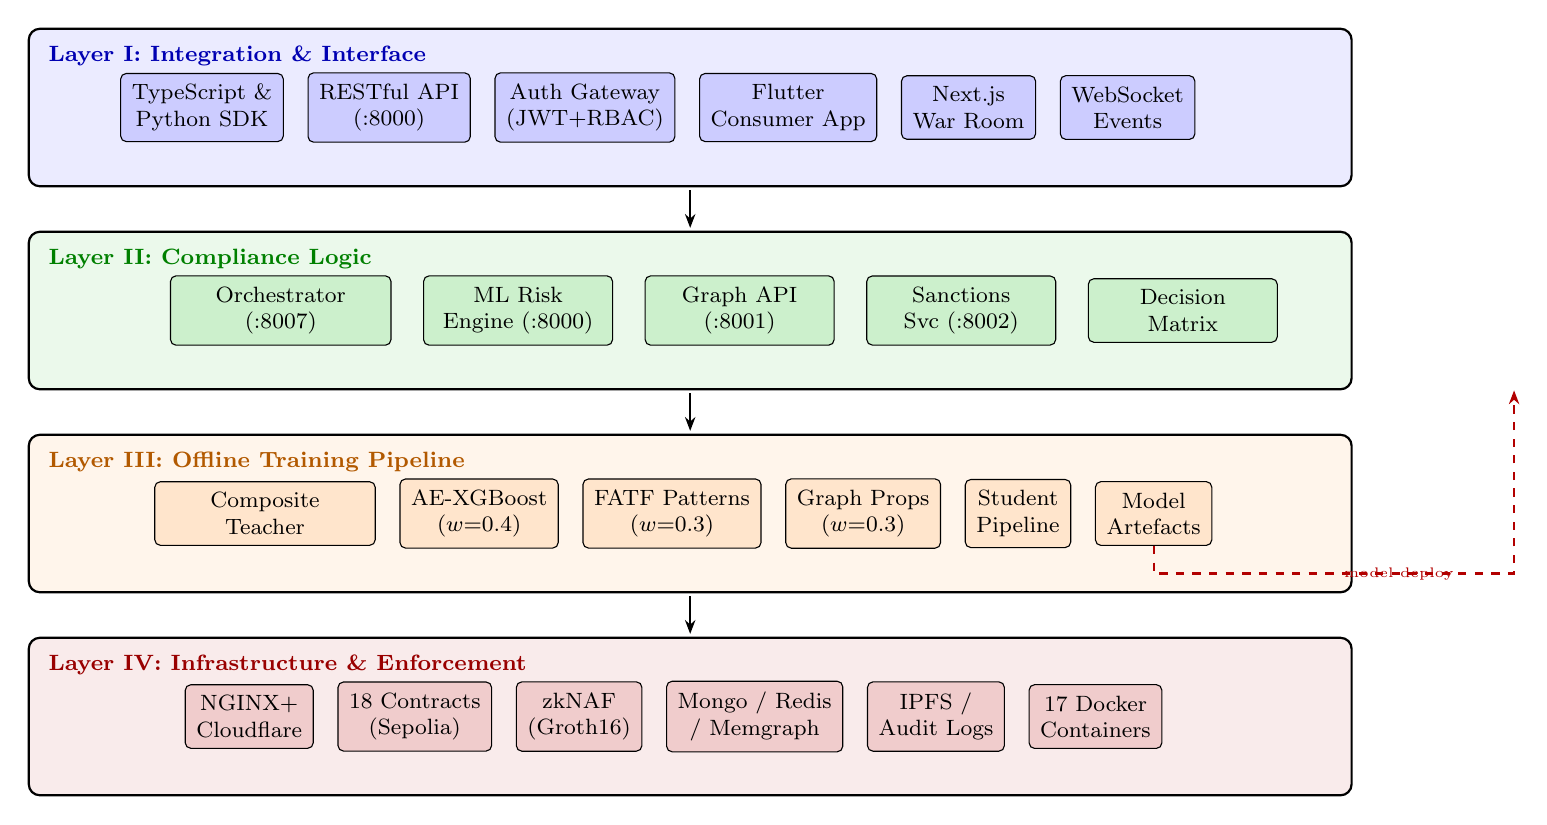
\begin{tikzpicture}[
    node distance=0.35cm and 0.3cm,
    every node/.style={font=\small},
    layer/.style={draw, rounded corners=4pt, minimum width=16.8cm, minimum height=2cm, fill=#1!8, thick},
    block/.style={draw, rounded corners=2pt, minimum height=0.75cm, fill=#1!20, font=\footnotesize, align=center, inner sep=4pt},
    arrow/.style={-{Stealth[length=5pt]}, thick},
    dasharrow/.style={-{Stealth[length=5pt]}, thick, dashed, red!70!black},
    lbl/.style={font=\footnotesize\bfseries, text=#1},
  ]

  % ---- Layer I ----
  \node[layer=blue] (L1) {};
  \node[lbl=blue!70!black, anchor=north west] at ([xshift=4pt, yshift=-3pt]L1.north west) {Layer I: Integration \& Interface};

  \node[block=blue] (sdk) at ([xshift=-6.2cm]L1.center) {TypeScript \&\\Python SDK};
  \node[block=blue, right=0.3cm of sdk] (rest) {RESTful API\\(:8000)};
  \node[block=blue, right=0.3cm of rest] (auth) {Auth Gateway\\(JWT+RBAC)};
  \node[block=blue, right=0.3cm of auth] (flutter) {Flutter\\Consumer App};
  \node[block=blue, right=0.3cm of flutter] (nextjs) {Next.js\\War Room};
  \node[block=blue, right=0.3cm of nextjs] (ws) {WebSocket\\Events};

  % ---- Layer II ----
  \node[layer=green!70!black, below=0.55cm of L1] (L2) {};
  \node[lbl=green!50!black, anchor=north west] at ([xshift=4pt, yshift=-3pt]L2.north west) {Layer II: Compliance Logic};

  \node[block=green!70!black, minimum width=2.8cm] (orch) at ([xshift=-5.2cm]L2.center) {Orchestrator\\(:8007)};
  \node[block=green!70!black, minimum width=2.4cm, right=0.4cm of orch] (mlrisk) {ML Risk\\Engine (:8000)};
  \node[block=green!70!black, minimum width=2.4cm, right=0.4cm of mlrisk] (graph) {Graph API\\(:8001)};
  \node[block=green!70!black, minimum width=2.4cm, right=0.4cm of graph] (sanctions) {Sanctions\\Svc (:8002)};
  \node[block=green!70!black, minimum width=2.4cm, right=0.4cm of sanctions] (matrix) {Decision\\Matrix};

  % ---- Layer III ----
  \node[layer=orange, below=0.55cm of L2] (L3) {};
  \node[lbl=orange!70!black, anchor=north west] at ([xshift=4pt, yshift=-3pt]L3.north west) {Layer III: Offline Training Pipeline};

  \node[block=orange, minimum width=2.8cm] (teacher) at ([xshift=-5.4cm]L3.center) {Composite\\Teacher};
  \node[block=orange, right=0.3cm of teacher] (aexgb) {AE-XGBoost\\($w{=}0.4$)};
  \node[block=orange, right=0.3cm of aexgb] (fatf) {FATF Patterns\\($w{=}0.3$)};
  \node[block=orange, right=0.3cm of fatf] (graphprop) {Graph Props\\($w{=}0.3$)};
  \node[block=orange, right=0.3cm of graphprop] (student) {Student\\Pipeline};
  \node[block=orange, right=0.3cm of student] (artefacts) {Model\\Artefacts};

  % ---- Layer IV ----
  \node[layer=red!70!black, below=0.55cm of L3] (L4) {};
  \node[lbl=red!60!black, anchor=north west] at ([xshift=4pt, yshift=-3pt]L4.north west) {Layer IV: Infrastructure \& Enforcement};

  \node[block=red!70!black] (nginx) at ([xshift=-5.6cm]L4.center) {NGINX+\\Cloudflare};
  \node[block=red!70!black, right=0.3cm of nginx] (contracts) {18 Contracts\\(Sepolia)};
  \node[block=red!70!black, right=0.3cm of contracts] (zknaf) {zkNAF\\(Groth16)};
  \node[block=red!70!black, right=0.3cm of zknaf] (data) {Mongo / Redis\\/ Memgraph};
  \node[block=red!70!black, right=0.3cm of data] (ipfs) {IPFS /\\Audit Logs};
  \node[block=red!70!black, right=0.3cm of ipfs] (docker) {17 Docker\\Containers};

  % ---- Arrows between layers ----
  \draw[arrow] ([yshift=-1pt]L1.south) -- ([yshift=1pt]L2.north);
  \draw[arrow] ([yshift=-1pt]L2.south) -- ([yshift=1pt]L3.north);
  \draw[arrow] ([yshift=-1pt]L3.south) -- ([yshift=1pt]L4.north);

  % ---- Dashed arrow: model artefact deployment ----
  \draw[dasharrow] (artefacts.south) -- ++(0,-0.35)
    -| ([xshift=3cm]matrix.east |- L2.south)
    node[pos=0.25, right, font=\tiny, text=red!70!black] {model deploy};

\end{tikzpicture}%
}% end resizebox
\caption{AMTTP four-layer architecture. Layer~I exposes integration interfaces; Layer~II implements compliance decision logic; Layer~III trains models offline via weak supervision; Layer~IV provides infrastructure and on-chain enforcement. The dashed arrow indicates model artefact deployment from the training pipeline to the production risk engine.}
\label{fig:architecture}
\end{figure*}

\subsection{Layer~I: Integration and Interface Layer}

Layer~I is the protocol's public surface. It exposes interfaces for human operators, third-party applications, and automated systems alike.

\textbf{AMTTP Open-Source SDK.} Using both TypeScript and Python as their respective client libraries for construction and signing of transactions, with WebSocket-enabled connections to keep rapidly streaming real-time events, and batched scoring interfaces if necessary to meet throughput requirements between them too.

\textbf{RESTful API Interface.} FastAPI service running on port 8000 which exposes production-compliance endpoints: \texttt{/score} endpoint evaluating individual transaction(s) against model-type(s), returning risk score(s) and accompanying reference-type metadata; \texttt{/batch} endpoint accepting arrays; \texttt{/model/info} endpoint providing metadata about model version \& features; \texttt{/alerts} endpoints provide feeds to SIEM dashboards; \texttt{/health} serves readiness probes.

\textbf{Web Application Layer.} Two distinct audiences are served by two separate web applications. The first, a consumer-oriented application developed using Flutter, connects to MetaMask and allows users to connect their wallets and review risk assessments before signing any agreements. The second, a Next.js based ``War Room'' dashboard, provides compliance analysts with access to live alerts, case management workflows, visualisation of scores, and a zkNAF proof verification panel.

\subsection{Layer~II: Compliance Logic Layer}

The Layer~II transaction processing system synthesises decisions. During data ingestion from Layer~I, the system checks the transaction data for risks using several Layer~II services concurrently, and the results are merged into one compliance decision.

\textbf{Compliance Orchestrator.} The Orchestrator directs parallel requests of incoming transactions into the ML Risk Engine, the Graph API, the Sanctions service, and the Geo-risk service. The responses are aggregated, enhanced by entity profile data, and framed into a unified risk assessment.

\textbf{Identity Management Module.} The Identity Management Module maintains entity profiles of KYC status, historical transaction patterns, jurisdictional metadata, and rules that will be used to evaluate each incoming transaction for compliance.

\textbf{Transaction Sequencing Module.} The Transaction Sequencing Module adds the context to transactions for compliance evaluation by appending to the transaction record: sanctions matches, KYC status, rule-based alerts, geographic risk, fraud probabilities, and confidence levels from the ML model prior to making a decision on the transaction.

\textbf{ML Risk Engine (Production CPU).} The production engine executes on a CPU-based infrastructure and retrieves artefacts of deployed models from a Docker volume; it uses the combined outputs from ensembles of the trained models of XGBoost and LightGBM, along with a logistic-regression meta-learner, to evaluate every incoming transaction.

\textbf{Compliance Decision Matrix.} The results of all signals are collated within the compliance decision matrix contained within Table~\ref{tab:decision_matrix}, whereby all signals are normalised to form one deterministic action matrix.

\begin{table}[!t]
\centering
\caption{Compliance Decision Matrix}
\label{tab:decision_matrix}
\begin{tabular}{p{5.2cm}l}
\toprule
\textbf{Condition} & \textbf{Action} \\
\midrule
risk $< 200$ $\land$ $\neg$sanctioned $\land$ geo $\neq$ PROHIBITED & APPROVE \\
$200 \leq$ risk $< 400$ $\land$ $\neg$sanctioned & APPROVE \\
$400 \leq$ risk $< 600$ $\land$ $\neg$sanctioned & REVIEW \\
$600 \leq$ risk $< 800$ & ESCROW \\
risk $\geq 800$ $\lor$ red flags & BLOCK \\
sanctioned $\lor$ FATF blacklist & BLOCK \\
velocity anomaly $\land$ risk $\geq 400$ & ESCROW \\
risk $> 600$ $\land$ $\neg$KYC & BLOCK \\
\bottomrule
\end{tabular}
\end{table}

\subsection{Layer~III: Offline Training Pipeline}

Layer~III is exclusively an offline process and is concerned only with creating and validating the machine-learning models that will be used by the production risk engine. Training occurs on GPU-based infrastructure (Google Colab) using a multi-stage weak supervision approach.

\textbf{Stage~1---Teacher Model (Hope Machine).} Data for training the Teacher Model (the Hope Machine) is derived from (2) publicly available Kaggle datasets: BitcoinHeist and Ethereum, with 2,640,911 rows over 177 features and a 0.87\% fraud rate (total class imbalance of 113 to 1), which is relatively conservative compared to real-world experiences.

\textbf{VAE Featurisation.} The VAEWithAttention model runs on GPU to produce latent vectors for the data with less complexity than the original feature set, yet still preserves the underlying data/relevant information. The reconstruction error from the VAE is also treated as an anomaly signal and is added directly to the feature set.

\textbf{Stage~2---Teacher Labelling.} The Teacher takes the form of a composite of (3) different types of teachers that were fused/combined and weighted together to create one composite pseudo-label:

\begin{itemize}
\item AE enhanced XGBoost ($w=0.4$) output on 1,670 fresh BigQuery transactions based on 171 engineered features and latent outputs derived from autoencoders;
\item FATF Pattern Detectors ($w=0.3$) generated using (7) behavioural rules that are based on AML typologies (\eg, SMURFING, FAN OUT, FAN IN, LAYERING, STRUCTURING, VELOCITY, and PEELING);
\item Graph-Structural Properties ($w=0.3$) derived from network study and analysis (\eg, degree centrality, community detection, handling of distance from verified illegitimate nodes).
\end{itemize}

The combination of the above (weighted) resulted in the pseudo-labels for the students' training to be produced.

\textbf{Stage~3a---Student VAE/GNN Pipeline.} This procedure allows a combined variational autoencoder (VAE) and graph neural network (GNN) to be trained using the pseudo-labels assigned to the student by the teacher. This is done using Colab's GPU infrastructure.

\textbf{Stage~3b---Production Models (CPU Deployed).} It's responsible for deploying the production models (CPUs) that were created in Stage~3a. Docker volumes are used to mount the model artefacts into the Layer~II risk engine, where they will be used as risk measures.

% ============================================================
%  Fig. 2 — ML Pipeline Diagram (TikZ)
% ============================================================
\begin{figure*}[!t]
\centering
\resizebox{\textwidth}{!}{%
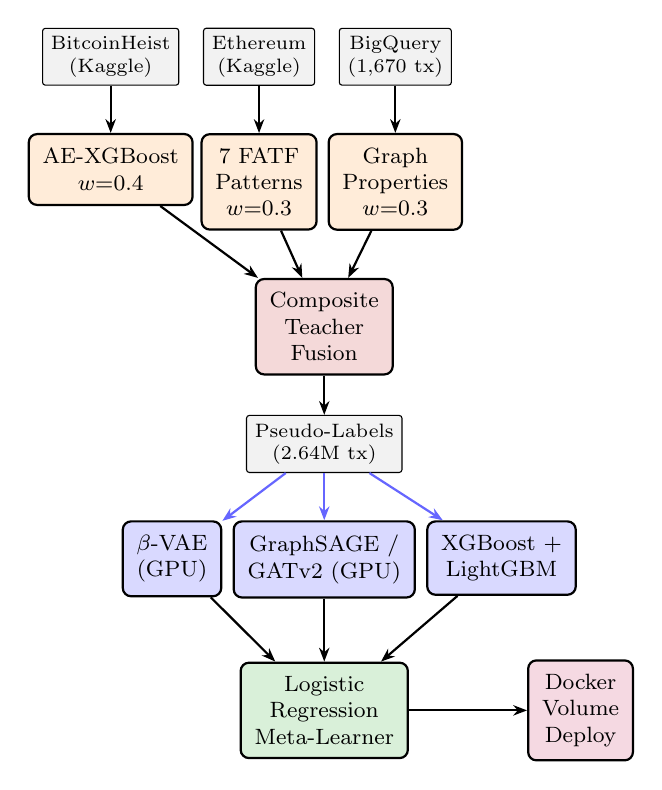
\begin{tikzpicture}[
    node distance=0.4cm and 0.5cm,
    every node/.style={font=\small},
    stage/.style={draw, rounded corners=3pt, minimum height=0.9cm, fill=#1!15, font=\footnotesize, align=center, inner sep=5pt, thick},
    data/.style={draw, rounded corners=1pt, minimum height=0.7cm, fill=gray!10, font=\scriptsize, align=center, inner sep=3pt},
    arrow/.style={-{Stealth[length=5pt]}, thick},
    warrow/.style={-{Stealth[length=5pt]}, thick, blue!60},
    lbl/.style={font=\tiny, text=gray!70!black},
  ]

  % ---- Data Sources ----
  \node[data] (btc) {BitcoinHeist\\(Kaggle)};
  \node[data, right=0.3cm of btc] (eth) {Ethereum\\(Kaggle)};
  \node[data, right=0.3cm of eth] (bq) {BigQuery\\(1,670 tx)};

  % ---- Teacher Components ----
  \node[stage=orange, below=0.6cm of btc] (aexgb) {AE-XGBoost\\$w{=}0.4$};
  \node[stage=orange, below=0.6cm of eth] (fatfp) {7 FATF\\Patterns\\$w{=}0.3$};
  \node[stage=orange, below=0.6cm of bq] (graphp) {Graph\\Properties\\$w{=}0.3$};

  % ---- Fusion ----
  \node[stage=red!70!black, below right=0.6cm and -0.8cm of fatfp] (fusion) {Composite\\Teacher\\Fusion};

  % ---- Pseudo-labels ----
  \node[data, below=0.5cm of fusion] (pseudo) {Pseudo-Labels\\(2.64M tx)};

  % ---- Student Pipeline ----
  \node[stage=blue, below left=0.6cm and 0.3cm of pseudo] (vae) {$\beta$-VAE\\(GPU)};
  \node[stage=blue, below=0.6cm of pseudo] (gnn) {GraphSAGE /\\GATv2 (GPU)};
  \node[stage=blue, below right=0.6cm and 0.3cm of pseudo] (xgblgb) {XGBoost +\\LightGBM};

  % ---- Meta-learner ----
  \node[stage=green!60!black, below=0.8cm of gnn] (meta) {Logistic\\Regression\\Meta-Learner};

  % ---- Deployment ----
  \node[stage=purple, right=1.5cm of meta] (deploy) {Docker\\Volume\\Deploy};

  % ---- Arrows ----
  \draw[arrow] (btc) -- (aexgb);
  \draw[arrow] (eth) -- (fatfp);
  \draw[arrow] (bq) -- (graphp);
  \draw[arrow] (aexgb) -- (fusion);
  \draw[arrow] (fatfp) -- (fusion);
  \draw[arrow] (graphp) -- (fusion);
  \draw[arrow] (fusion) -- (pseudo);
  \draw[warrow] (pseudo) -- (vae);
  \draw[warrow] (pseudo) -- (gnn);
  \draw[warrow] (pseudo) -- (xgblgb);
  \draw[arrow] (vae) -- (meta);
  \draw[arrow] (gnn) -- (meta);
  \draw[arrow] (xgblgb) -- (meta);
  \draw[arrow] (meta) -- (deploy);

\end{tikzpicture}%
}% end resizebox
\caption{Layer~III offline training pipeline. Two public datasets feed the composite teacher: autoencoder-enhanced XGBoost predictions ($w{=}0.4$), FATF typology pattern detectors ($w{=}0.3$), and graph-structural properties ($w{=}0.3$) are fused into pseudo-labels. The student pipeline---VAE/GNN and gradient boosted classifiers---trains on these labels, unified by a logistic regression meta-learner and deployed to the production risk engine.}
\label{fig:pipeline}
\end{figure*}

\subsection{Layer~IV: Infrastructure and Enforcement Layer}

The infrastructure and enforcement layers provide a bridge between off-chain compliance verdicts and on-chain enforcement to ensure compliance with legal and regulatory obligations.

\textbf{API Gateway.} The API Gateway includes an NGINX reverse proxy that handles TLS termination, rate limiting to 100 requests per second, and path-based routing, as well as a Cloudflare Tunnel that supplies the secure connection from outside the public Internet.

\textbf{On-Chain Verification---Ethereum Smart Contracts.} 18 Ethereum smart contracts written in Solidity are deployed on the Ethereum Sepolia blockchain (shown in Table~\ref{tab:contracts}).

\begin{table}[!t]
\centering
\caption{AMTTP Smart Contract Components}
\label{tab:contracts}
\begin{tabular}{ll}
\toprule
\textbf{Contract} & \textbf{Purpose} \\
\midrule
AMTTPCore & Risk oracle, escrow, threshold sigs \\
AMTTPNFT & KYC badges (ERC-721) \\
DisputeResolver & Kleros arbitration integration \\
CrossChain & LayerZero cross-chain relay \\
PolicyEngine & Rule \& threshold configuration \\
RiskRouter & Multi-chain score routing \\
zkNAFVerifier & Groth16 proof verification \\
SafeModule & Gnosis Safe multi-sig \\
CoreSecure & Hardened variant, reentrancy guards \\
Streamlined & Gas-optimised compliance \\
BiconomyModule & Gasless meta-transactions \\
PolicyManager & Policy \& threshold management \\
\bottomrule
\end{tabular}
\end{table}

\textbf{zkNAF Circuits.} Three types of proof are provided for compliance verification: KYC Credential Proofs, Risk Range Proofs, and Non-Membership Proofs (shown in Table~\ref{tab:zknaf}).

\begin{table}[!t]
\centering
\caption{zkNAF Proof Types}
\label{tab:zknaf}
\begin{tabular}{p{2.8cm}p{4.8cm}}
\toprule
\textbf{Proof Type} & \textbf{Purpose} \\
\midrule
KYC Credential & Verify identity status without revealing personal data \\
Risk Range & Prove risk score within acceptable bounds without disclosing exact value \\
Sanctions Non-Membership & Confirm address is not on watchlists without exposing the full list \\
\bottomrule
\end{tabular}
\end{table}

\textbf{Data Persistence Layer.} The various data storage technologies provide distinct functionalities:

\begin{itemize}
\item MongoDB stores entity profiles, alerts, transaction history, and audit trails.
\item Redis provides in-memory sessions, rate limits for sending, and sender feature vector caching.
\item Memgraph is used for the graph layer: entity relationships and risk propagation paths.
\item Helia/IPFS provides immutable audit logs, evidence packages, and cryptographic proof records.
\item BigQuery is used for ingestion of training data for 30 days' worth of Ethereum transactions, 30 days' worth of Ethereum transaction records (approximately 1.67 million records total).
\end{itemize}

% ============================================================
%  IV. PRODUCTION IMPLEMENTATION
% ============================================================
\section{Production Implementation}

The entire system ships as a containerised deployment, orchestrated through Docker Compose. Table~\ref{tab:services} catalogues the 17 services, their ports, and their principal functions.

\begin{table}[!t]
\centering
\caption{AMTTP Service Infrastructure}
\label{tab:services}
\begin{tabular}{llll}
\toprule
\textbf{Service} & \textbf{Port} & \textbf{Purpose} & \textbf{Tech} \\
\midrule
NGINX Gateway & 8888 & Reverse proxy, TLS & NGINX \\
Flutter App & 8889 & End-user interface & Flutter \\
Next.js War Room & 3006 & Compliance dashboard & Next.js \\
Orchestrator & 8007 & Decision coord. & FastAPI \\
ML Risk Engine & 8000 & Risk scoring & FastAPI \\
Graph API & 8001 & Memgraph interface & FastAPI \\
Sanctions Svc & 8002 & Watchlist screening & FastAPI \\
Entity Profiler & 8003 & KYC management & FastAPI \\
Geo-Risk Svc & 8004 & Geographic risk & FastAPI \\
Alert Manager & 8005 & Alert routing & FastAPI \\
Auth Service & 8020 & Authentication & FastAPI \\
MongoDB & 27017 & Document store & MongoDB \\
Redis & 6379 & In-memory cache & Redis \\
Memgraph & 7687 & Graph database & Memgraph \\
Helia/IPFS & 5001 & Immutable storage & Helia \\
Prometheus & 9090 & Metrics collection & Prom. \\
Grafana & 3000 & Dashboards & Grafana \\
\bottomrule
\end{tabular}
\end{table}

% ============================================================
%  V. SECURITY MODEL
% ============================================================
\section{Security Model}

There are many layers of security controls throughout the architecture. The API Gateway at the edge of the architecture provides TLS termination as well as rate limiting to a maximum of 100 requests/sec, while Cloudflare Tunnel provides external access security to the architecture at the edge. The UI Integrity Service verifies no tampering with the front end.

The smart contract suite incorporates multi-signature governance using a safe module, allowing for M-of-N methods of approval for privileged operations. CoreSecure and Streamlined, which are hardened and gas-optimised versions of the same contract, have both been built with reentrancy protection using the OpenZeppelin audited library~\cite{openzeppelin2024}.

Three types of proof are used in the zkNAF to complete the security model. See Table~\ref{tab:zknaf} for more detail.

% ============================================================
%  VI. EVALUATION AND BENCHMARKS
% ============================================================
\section{Evaluation and Benchmarks}

The evaluation of AMTTP consists of six evaluations: ML Model Performance, Cross-Level Generalisation, Score Recalibration, External Validation on Independent Datasets, Smart Contracts Gas Costs and System-Level Integration. The measurements used were from the Production Pipeline, defined in Sections~\ref{sec:arch} and~IV.

\subsection{Machine Learning Model Performance}

Production Pipeline V2 is made up of different stages. $\beta$-VAE trained (using only normal addresses---468,564 samples) provides latent embedding (anomaly) scores. The transaction graph used contains 625,168 nodes and 1,673,244 edges for building structural embedding (GraphSAGE---3 layer, 128 dimension, GATv2-4 head attention). The GNN structural embeddings were concatenated, and then PCA was applied to compress from 192 dimensions into 45 dimensions (98.3\% variance retained). The resulting embeddings created from Optuna-tuned XGBoost and LightGBM classifiers wired together via a logistic regression meta-learner provide the final probabilities for fraud detection. The performance of components and ensemble (Table~\ref{tab:v2perf}---Performance on actual test set of held-out test addresses) was assessed on a held-out (125,034 addresses---25.05\% fraud rate) test set.

\begin{table}[!t]
\centering
\caption{V2 Pipeline Component Performance (Test Set, $n = 125{,}034$)}
\label{tab:v2perf}
\begin{tabular}{lcc}
\toprule
\textbf{Component} & \textbf{ROC-AUC} & \textbf{PR-AUC} \\
\midrule
$\beta$-VAE (recon.\ error) & 0.8290 & 0.5387 \\
$\beta$-VAE (Mahalanobis) & 0.7435 & 0.4550 \\
GATv2 & 0.9968 & 0.9916 \\
GraphSAGE & 0.9994 & 0.9984 \\
XGBoost (OOF) & 0.9999 & 0.9998 \\
LightGBM (OOF) & 0.9999 & 0.9998 \\
Meta-Ensemble & 1.0000 & 0.9999 \\
\bottomrule
\end{tabular}
\end{table}

The meta-ensemble achieved an impressive ROC-AUC of 1.0000 and a PR-AUC of 0.9999; however, these results were nested within an overarching predictable set of previously constructed labels as they were generated as part of the teacher's weak supervision pipeline using a so-called ``proxy'' level (or, more accurately, a proxy level for what the teacher created). Since the student is being evaluated against a distribution as to what it should be, this is a valid test for the determination of whether the model output corresponds to the desired output. A more sober estimate of the generalisability rate can be obtained from the five-fold cross-validation results derived from the 372 independently verified fraud addresses: the Student-XGBoost ROC-AUC score was 0.9957 (see \S\ref{sec:crossval} for detailed study information). One aspect of this experiment that is particularly noteworthy is that the ratio of $\beta$-VAE reconstruction output error for fraud and normal addresses (0.1550 vs.\ 0.0595) was 2.60$\times$. This indicates that, while the autoencoder did not have the benefit of seeing a single fraud account during training, it was able to identify these accounts as being out of distribution, which is very encouraging.

\subsection{Five-Fold Cross-Validation}
\label{sec:crossval}

A single train--test split does not demonstrate how well a model generalizes. For this reason, we also applied five-fold stratified cross-validation to the entire 625,168 unique address dataset (372 verified fraud addresses with fraud rates of 0.06\%). The Student-XGBoost base model results per fold are detailed in Table~\ref{tab:cv}.

\begin{table}[!t]
\centering
\caption{Five-Fold Cross-Validation (625,168 Addresses, 372 Fraud)}
\label{tab:cv}
\begin{tabular}{lccc}
\toprule
\textbf{Fold} & \textbf{ROC-AUC} & \textbf{PR-AUC} & \textbf{Time (s)} \\
\midrule
1 & 0.9990 & 0.7047 & 164.1 \\
2 & 0.9994 & 0.6317 & 145.7 \\
3 & 0.9982 & 0.6721 & 175.8 \\
4 & 0.9986 & 0.6876 & 147.1 \\
5 & 0.9873 & 0.5971 & 52.1 \\
\midrule
Mean $\pm$ SD & $0.9965 \pm 0.0049$ & $0.6586 \pm 0.0404$ & 136.9 \\
\bottomrule
\end{tabular}
\end{table}

The average ROC-AUC and PR-AUC for the student XGBoost over the five cross-validation folds are 0.9965 ($\pm$0.0049) and 0.6586 ($\pm$0.0404), respectively. When aggregating the out-of-fold predictions, we obtain an ROC-AUC and PR-AUC of 0.9957 and 0.6333, respectively, with an F1 of 0.635 at the optimal threshold. The agreement on the prediction between the teacher and student is at 99.27\%.

\subsection{Teacher Model and Knowledge Distillation}

The teacher model is a hybrid of a fully autoencoder enhanced XGBoost algorithm, FATF pattern detectors, and weighted graph structure properties (0.4/0.3/0.3) trained on 2,640,911 labelled samples from BitcoinHeist and Ethereum Kaggle with a class ratio of 113:1. The teacher's test PR-AUC and ROC-AUC values are 0.6491 and 0.9255, respectively. By separating into blockchain type, we see a significant difference in performance between the two blockchains. The Ethereum PR-AUC is 0.9517 while the Bitcoin's PR-AUC is only 0.6091. The disparity traces to the sparser feature set available for Bitcoin addresses.

Distillation quality is assessed through calibration and divergence metrics. The student meta-ensemble achieves a Brier score of 0.000718 on the 125,034-address test set, against the teacher's 0.1898. Jensen--Shannon divergence between the two score distributions sits at 0.1601---moderate, and consistent with the student having learnt a crisper decision boundary than its teacher.

\subsection{Transaction-Level Evaluation}

AMTTP also trains models at transaction granularity across 1,673,244 records. TX-Level XGBoost: ROC-AUC 0.9878, PR-AUC 0.9713. TX-Level LightGBM: ROC-AUC 0.9876, PR-AUC 0.9707. Their ensemble: ROC-AUC 0.9879, PR-AUC 0.9715, F1 of 0.901, precision 0.927, recall 0.877.

\subsection{Cross-Level Generalisation}

One of the long-standing problems that have existed for AML systems in production is the difference in level of detail that the model was trained on and will score against. For example, the V2 Student models were trained using the aggregated data from address level, consisting of 625,168 addresses, with 71 feature inputs to the model (5 tables, 64 $\beta$-VAE latent embeddings, reconstruction error, and GraphSAGE score) whereas production scores will occur on a transaction level. The profiling of those systems indicated a significant training to serving skew; of the 71 features used to train the models, only 5 could be calculated from a raw transaction coming to the API. The 66 remaining features, including all of the deep learning embedding features, were all 0. At inference time, 93\% of the model's inputs were 0s, resulting in reduced performance; Student v2 XGBoost performance dropped to ROC-AUC of .6436 and F1 score of .483.

The solution we have implemented is Path~B, where the models have been developed and retrained directly against transactions, using a smaller set of features, with 21 guaranteed to exist at inference time; 6 taken directly from the API Transaction Request, 7 derived arithmetically, and 8 sender-history features drawn from an address index cache (all default to 0 gracefully if they do not exist). The labels are propagated from address-level ground truth information at the address level through the sender's account join, meaning that if an address is labelled as being fraudulent, all transactions going through that address will inherit that label as well. Through this methodology, we created a total of 420,848 transactions that were labelled fraudulent, with a total of 1,673,244 transactions being evaluated (or 25.15\%). A summary of the comparison of the two can be found in Table~\ref{tab:crosslevel}.

\begin{table}[!t]
\centering
\caption{Cross-Level Generalisation: Address vs.\ Transaction Models}
\label{tab:crosslevel}
\begin{threeparttable}
\begin{tabular}{lccccc}
\toprule
\textbf{Model} & \textbf{ROC} & \textbf{PR} & \textbf{F1} & \textbf{Prec.} & \textbf{Rec.} \\
\midrule
Teacher Stack\tnote{$\dagger$} & .730 & .690 & .700 & 1.00 & .539 \\
Student v2 XGB & .644 & .362 & .483 & .414 & .581 \\
Student v2 Ens. & .632 & .349 & .473 & .396 & .587 \\
TX-Level XGB & .988 & .971 & .901 & .921 & .882 \\
TX-Level LGB & .988 & .971 & .899 & .925 & .873 \\
TX-Level Ens. & .988 & .972 & .901 & .927 & .877 \\
\bottomrule
\end{tabular}
\begin{tablenotes}
\item[$\dagger$] Circular: teacher evaluated on data it labelled.
\end{tablenotes}
\end{threeparttable}
\end{table}

The data speaks for itself---TX-Level XGBoost has an ROC-AUC of 0.9878 compared to the 0.6436 achieved by the address-level Student v2 XGBoost, resulting in a total delta of 0.344. The F1 score increased from 0.483 to 0.901. Inference is assured to contain exactly the same features that were used for training (there is zero degree of training--serving skew). Furthermore, the meta-learner has collapsed down to a logistic regression (with respect to the XGBoost and LightGBM probabilities as inputs), that has coefficients of 7.74 and 2.22, and an intercept value of $-6.25$, thus eliminating all of the GPU and graph dependencies associated with real-time scoring.

\subsection{Score Recalibration}

The probabilistic outputs of raw models are inadequate indicators of risk. The output probabilities from the teacher (XGBoost) have been compressed into a very narrow range of probabilities (0\% to 1.1\%). The optimal F1 score threshold for the model is 0.0027 even though its ROC-AUC value is 0.9969. However, the issue can be resolved using a two-stage recalibration pipeline. First, create a sigmoid transformation centered at the 75th percentile (P75) of output probabilities, with a steepness $k = 30$:
\begin{equation}
p_{\text{cal}} = \frac{1}{1 + \exp\!\bigl[-k \cdot (x - P_{75})\bigr]}
\label{eq:recalibration}
\end{equation}
The resulting optimal F1 score threshold will be 0.5199, which is a reasonable value, but the ranking of each record will still be preserved (no change in the ROC-AUC value of 0.9969). Second, normalize the transformed output probability via percentile rank mapping onto a 0 to 100 scale for the user's descriptive consumption. Using the following designations for the percentiles of top records: CRITICAL (top 1\% of records and P99), HIGH (top 5\% of records and P95), MEDIUM (top 15\% of records and P85), LOW (top 30\% of records and P70), and MINIMAL (all remaining records). The original production threshold of 0.96 now appears to have been an overly conservative estimate because nearly all records for which an address was flagged passed all screening tests. The recalibrated threshold for blocking transactions will be reduced to 0.50; for escrow, to 0.65; and for review to 0.50. Each of the nine BEHAVIOURAL PATTERN BOOSTS will add an additive increment in the score of the respective record: SMURFING and STRUCTURING, each with +25\%; PEELING, +20\%; LAYERING (+15\%); and both FAN OUT and FAN IN, with +15\% and +10\% respectively. In addition to the above, there will be further GRAPH BASED PROXIMITY BOOST adjustments (+40\% for DIRECT sanctioned connections), and (+20\% for 2-HOP). If multiple detection CHANNELS converge, then an adjustment factor of (1.2$\times$ for 2 signals from the same channel and 1.5$\times$ for 3 signals from the same channel) is applied through a QUANTITATIVE application of the DEFENCE-IN-DEPTH principle.

\subsection{External Validation}

The ultimate test of the model's generalisability is its ability to perform well when presented with data it has not trained on. We assess the V2 pipeline using three separate external datasets that have been validated independently using a multi-strategy approach: (A)~XGBoost with zero-padded feature alignment; (B)~the entire V2 pipeline, calibrated with Platt recalibration, using a 20\%~calibration/80\%~evaluation split; (C)~the application of Meta-LR using Platt scaling; and (D)~concept alignment by appending the V2 score to the dataset as an additional feature and performing five-fold cross-validated logistic regression on the transactional-level features of the target dataset; (E)~reinforcement learning using ML3 with Platt correction for all evaluation scores based on the original distribution of the training data.

The most rigorous of these tests will involve using the Elliptic Bitcoin data set (comprising of 46,564 labelled transactions, of which 4,545 were considered to be fraudulently labelled as illicit, verified as being correct by Law Enforcement) to cross-check the predictions made by our distinct student system that was trained using Ethereum data that has been pseudo annotated by a Teacher and 99.7\% of which was trained using the BitcoinHeist dataset. Thus, the use of knowledge distillation provides a bridge across both the blockchain and labelling methodologies. Additionally, we will be using the XBlock Ethereum phishing dataset (comprising of 9,841 addresses, of which 2,179 have been verified to be phishing attempts by Zhejiang University) to conduct cross-modal generalisation, where address-level labels are generated by a transactional level prediction model and aggregated by transaction type (\eg, sender/receiver). The Forta Network dataset shows that both the teacher and the student produced results that were below the ROC-AUC of 0.5, but that does not mean there is a defect in the models. It indicates a semantic discrepancy between the behavioral fraud signatures identified with AMTTP and the threat taxonomy defined by Forta based on intelligence. In addition to the semantic differences between the models, the distribution of the two datasets is also different: The mean of the gas price in the training dataset is 1.1 gwei, while the mean is 42.4 gwei in the Forta dataset, and the mean number of transactions sent by addresses in the training dataset is 2,833 transactions as opposed to 40 transactions.

\subsubsection{Recalibration and Feature Enrichment}

The features in the external datasets do not line up exactly with those from the training data, so a reconstruction step followed by scoring is used before the scoring process. The reconstructed address will be fed into the XBlock pipeline to produce 7 separate FATF behavioral patterns from the available address aggregates. The 7 scores will then be combined into one score (for example, one from the Teacher XGBoost [$0.4\times$Teacher XGB $+\;0.3\times$Pattern Score $+\;0.3\times$Sophisticated]) with the Behavioral Patterns (XBlock) appended and before determining where the address falls within the Toxicity distribution. The coverage of the TX-Level models will increase from 9/21 to 14/21. The number of Student v2 tabular features will increase from 3/5 to 5/5. In order to unlock latent ranking capabilities, the adaptive percentiles used during the scoring process will use the model's score distribution to determine its percentiles rather than a fixed cut-off. Additionally, Platt re-calibration will use a logistic regression model to fit the raw probability scores to calibrated probabilities on a range of $[0,1]$ from the held out portion of the dataset.

The recalibration and feature enrichment outcomes from all five model generations and datasets are recorded in Table~\ref{tab:recalibration}. The 3 post-hoc adjustments used for all cases were the following: (1)~Platt re-calibrated; (2)~FATF pattern enriched; and (3)~Adaptive percentile thresholds. Each row contains information on the ROC AUCs and the best possible F1 scores associated to the particular correction made.

The best possible outcome per dataset-domain relationship intervention is shown for each database in Table~\ref{tab:crossdomain}.

% ============================================================
%  Table VIII — Recalibration Results (landscape, full-width)
% ============================================================
\begin{table*}[!t]
\centering
\caption{Recalibration and Feature Enrichment Results Across External Datasets}
\label{tab:recalibration}
\scriptsize
\begin{tabular}{llccccl}
\toprule
\textbf{Dataset} & \textbf{Model / Strategy} & \textbf{Raw ROC} & \textbf{Raw F1} & \textbf{Corr.\ ROC} & \textbf{Corr.\ F1} & \textbf{Correction Applied} \\
\midrule
\multicolumn{7}{l}{\textit{Elliptic --- Cross-Chain (Bitcoin $\to$ Ethereum student, $n = 46{,}564$, 9.8\% illicit)}} \\
\cmidrule(l){1-7}
Elliptic & Student XGB (zero-padded) & 0.7808 & 0.5999 & --- & --- & Baseline (best raw) \\
Elliptic & Full Pipeline + Platt & 0.7009 & 0.2954 & 0.7009 & 0.2946 & Platt recalibration \\
Elliptic & Meta-LR + Platt & --- & --- & 0.7176 & 0.3909 & Platt recalibration \\
Elliptic & ML3-RL + Platt & --- & --- & 0.6526 & 0.2498 & Platt recalibration \\
Elliptic & Teacher XGB & 0.4505 & 0.2121 & 0.5513 & 0.2246 & Platt recalibration \\
Elliptic & Concept Alignment (D) & 0.9311 & --- & 0.9334 & --- & V2 score appended to 166 features \\
\midrule
\multicolumn{7}{l}{\textit{XBlock --- In-Domain Ethereum, Cross-Level (address $\to$ tx model, $n = 9{,}841$, 22.1\% phishing)}} \\
\cmidrule(l){1-7}
XBlock & Student XGB (zero-padded) & 0.2922 & 0.3630 & 0.7111 & 0.5210 & Platt recalibration \\
XBlock & Meta-LR + Platt & --- & --- & 0.6030 & 0.4371 & Platt recalibration \\
XBlock & ML3-RL + Platt & --- & --- & 0.6744 & 0.4676 & Platt recalibration \\
XBlock & Teacher XGB & 0.4086 & 0.3860 & 0.5927 & 0.4528 & Platt recalibration \\
XBlock & Teacher XGB (percentile) & --- & --- & 0.7492 & 0.5288 & Adaptive percentile (P39.4) \\
XBlock & Student XGB orig (3/71) & 0.6507 & 0.4669 & 0.3740 & 0.3865 & +FATF enrichment (5/71) \\
XBlock & Student LGB orig (3/71) & 0.4058 & 0.3810 & 0.3620 & 0.3873 & +FATF enrichment (5/71) \\
XBlock & TX-Level XGB (9/21) & 0.5833 & 0.3838 & 0.6276 & 0.4037 & Feature enrichment (14/21) \\
XBlock & TX-Level LGB (9/21) & 0.6385 & 0.4407 & 0.6562 & 0.4387 & Feature enrichment (14/21) \\
XBlock & TX-Level Ens (9/21) & 0.6024 & 0.3953 & 0.6454 & 0.4160 & Feature enrichment (14/21) \\
XBlock & ML+FATF 60/40 blend & --- & --- & 0.4055 & --- & Combined ML + FATF \\
XBlock & OR-union (ML+Rules+FATF) & --- & --- & --- & 0.3626 & Multi-layer union \\
\midrule
\multicolumn{7}{l}{\textit{Forta --- Out-of-Domain (semantic mismatch, $n = 289$)}} \\
\cmidrule(l){1-7}
Forta & Student v2 & 0.1512 & --- & --- & --- & No correction effective \\
Forta & Teacher XGB & 0.2121 & --- & --- & --- & No correction effective \\
\midrule
\multicolumn{7}{l}{\textit{Etherscan --- Sanity Check ($n = 23$, 3 fraud / 20 clean)}} \\
\cmidrule(l){1-7}
Etherscan & Production pipeline & 0.4417 & 0.50 & --- & --- & Precision = 1.0, 0 false positives \\
\midrule
\multicolumn{7}{l}{\textit{Out-of-Domain Benchmarks --- Zero Feature Overlap with Training Distribution}} \\
\cmidrule(l){1-7}
Credit Card & Student XGB (93$\to$28 PCA) & --- & --- & --- & --- & 0\% recall; all fraud missed \\
Shuttle & Student XGB (93$\to$9 telemetry) & --- & --- & 0.316 & --- & 71.1\% recall, extreme false alarms \\
Mammography & Student XGB (93$\to$6 radio.) & --- & --- & --- & --- & 0\% recall; trivial all-clean \\
Pendigits & Student XGB (93$\to$16 digit) & --- & --- & --- & --- & 0\% recall; trivial all-clean \\
\bottomrule
\end{tabular}
\end{table*}

\begin{table}[!t]
\centering
\caption{Cross-Domain Performance Summary}
\label{tab:crossdomain}
\scriptsize
\begin{tabular}{lccl}
\toprule
\textbf{Dataset} & \textbf{Best ROC} & \textbf{Best F1} & \textbf{Domain Relationship} \\
\midrule
Elliptic & 0.7808 & 0.600 & Cross-chain (BTC$\to$ETH) \\
Elliptic (D) & 0.9334 & --- & +Concept alignment \\
XBlock & 0.7492 & 0.529 & In-domain, cross level \\
XBlock (union) & --- & 0.363 & +Multi-layer (99.8\% recall) \\
Forta & 0.1512 & --- & Semantic mismatch \\
Etherscan & --- & 0.500 & Sanity check ($n = 23$) \\
\midrule
\multicolumn{4}{l}{\textit{Out-of-domain (zero feature overlap):}} \\
Credit Card & --- & 0.000 & Banking (PCA, $n$=284,807) \\
Shuttle & --- & 0.316 & Aerospace ($n$=49,097) \\
Mammography & --- & 0.000 & Medical ($n$=11,183) \\
Pendigits & --- & 0.000 & Digit recog.\ ($n$=6,870) \\
\midrule
\multicolumn{4}{l}{\textit{V1 baselines (pre-distillation, no corrections):}} \\
Elliptic V1 & 0.3484 & 0.180 & TX-Level Ens v1.0 \\
XBlock V1 & 0.6024 & 0.396 & TX-Level Ens v1.0 \\
\bottomrule
\end{tabular}
\end{table}

\subsubsection{Key Observations}

To further evaluate the robustness of the domain boundaries, we have tested Student XGB against four completely different benchmark data sets: Credit Card Fraud (banking, PCA-transformed, $n$=284,807, 0.17\% fraud incidence; Dal Pozzolo et al.\ (2015)), Shuttle (NASA telemetry anomaly, $n$=49,097, 7.15\% incidence; ODDS), Mammography (radiological anomaly, $n$=11,183, 2.32\% incidence; Woods et al., 2014); Pendigits (handwritten digit anomaly; $n$=6,870, 2.27\% incidence; Alimoglu, 1996). All features have been matched to the 93~feature AMTTP scheme using positional mapping; any positional mismatches have been zero-padded. In three of the four datasets, the model produces 0~recall---when an anomaly is identified or ``found'' an anomaly has been missed the remainder of the anomalies. In only one instance, the Shuttle dataset yielded a limited recall of 71.1\%, however the false positive rate at 0.318 is unrecoverable making its utility very low. The zero recalls are not surprising. Student XGB has never been trained using PCA-transformed transactional banking data, telemetry data from a radiator or pen-stroke data. No recalibration or enrichment of the features used could be applied because the seven FATF-based patterns of behavior, structural characteristics of the graph or the blockchain-based aggregates/patterns of transactions, do not exist in either domain. Therefore the zero recalls from Student XGB represent the total and unequivocal failure of the application to produce meaningful results against the benchmark data-sets and provide further evidence that the distilled representations of AMTTP are behavioral semantics of financial transactions not generic structure of the anomaly detected.

The XBlock student XGBoost model (XGB) had a raw ROC-AUC value of 0.2922. This value is lower than what you would expect to achieve when simply guessing which were legitimate transactions, and the ROC-AUC value cannot be used in this case any longer because all of the model's probability values cluster in a small window of $[0.0008, 0.0032]$. The model's performance improves significantly if the Platt recalibration method is applied to it, such that the ROC-AUC becomes 0.7111 (+0.4189), which represents the largest single increase in performance we have observed. The teacher XGB had even lower probability values ranging from 0.000256--0.000401. Despite this, we were able to recover both the ROC-AUC (0.7492) and F1 (0.5288) using the adaptive percentile thresholding method for 39.4\% of the observations. This indicates that although the relative ranking of models has been preserved with respect to fraud detection versus legitimate transactions, the absolute probability calibration has broken down. The concept of appending the V2 score as an additional feature to each of Elliptic's (166) native features has improved both the ROC-AUC from 0.9311 to 0.9334 as well as the PR-AUC from 0.6241 to 0.6481. Therefore, a very small amount of information related to the cross-chain analysis provides considerable value when combined with an already rich dataset. Finally, our multi-layer coverage analysis results for the XBlock demonstrate that we have achieved a total of 99.8\% recall on all 2,179 examination phishing address records when aggregating machine learning (ML), rule-based, and Financial Action Task Force (FATF) pattern methods. Furthermore, of the 22 total fraud cases that our best ML technique was unable to detect, 22 were successfully detected using either rule-based or FATF pattern methods.

A smaller sanity check substantiates directional validity. Twenty-three Ethereum addresses---three independently confirmed fraudulent via Etherscan---are scored by the production pipeline. At the CRITICAL-or-HIGH threshold, precision is 1.0, recall 0.333 (F1~$=$~0.50), with zero false positives on the 20 clean addresses.

\subsubsection{Inferences on Generalisation and Knowledge Distillation}

Seven inferences emerge from these results.

\begin{enumerate}
\item \textbf{Knowledge distillation transfers ranking, not calibration.} It only transfers rankings. In models where the student was trained to compare two addresses for fraud (and thus developed an ordering of the addresses based on likely fraud), this ordering holds regardless of whether the student is used to score the two addresses in an external environment (\ie, across-blockchain or at different transaction levels). However, while the student's ordering of addresses remains the same across environments, the absolute probability for each address is collapsed; raw probability scores are compressed into a near-zero range. Nevertheless, the student can recover the full discriminative power of the model through post-hoc Platt recalibration (also known as ``calibration'') and/or through percentile normalisation (\ie, converting the student's raw score into the corresponding percentile). This finding is consistent across all three generations of models evaluated, and for external datasets where the semantic domain of the student and the teacher's datasets align.

\item \textbf{Feature sparsity determines the enrichment ceiling.} TX-Level models (with 9 out of 21 possible features mapped) achieve consistent gains in ROC-AUC (Area Under the Receiver Operating Characteristic) through the addition of features up to 14 out of 21 possible features (XGB~$=$~+0.044, LGB~$=$~+0.018, Ensemble~$=$~+0.043). In contrast, student (V2) models (with 3 out of 71 possible features mapped) fail to improve as additional features are added (the addition of two more features results in 5 total mapped; however, the 66 remaining features are blank and provide no useful signal); the student has a 93\% zero-sparsity score (or nearly no features with valid signals), meaning enrichment at this level of sparsity cannot be achieved.

\item \textbf{Cross-chain generalisation exceeds expectations.} The student is trained using only Ethereum pseudo-labels but achieves 0.7808 ROC-AUC on the Elliptic Bitcoin Dataset, which it had never previously encountered. This score exceeds the baseline of 0.3484 for the V1 TX-Level model ensemble and, therefore, indicates that the distilled feature representations developed by the student encapsulate semantics related to fraud that exists within both blockchain and non-blockchain networks, thereby establishing that the student can generalise across blockchains.

\item \textbf{Semantic alignment is a prerequisite; no correction can bridge a taxonomy mismatch.} The model does not perform well on five of the nine external testing datasets (Forta [ROC-AUC~$=$~0.15]; Credit [F1~$=$~0.000]; Shuttle [F1~$=$~0.316]; Mammography [F1~$=$~0.000]; and Pendigits [F1~$=$~0.000]). Forta fails to match AMTTP's behavioural fraud identifiers with the outputs of its threat intelligence-based labelling, while the other four out-of-domain validation benchmarks are also mismatched with the blockchain transaction variables. The relationship between the features of the two types is clear; distilled representations can be transferred across chains (as in Elliptic) and across different levels of abstraction (as in XBlock), but cannot be transferred across fundamentally dissimilar feature ontologies. The evidence of the five dataset failure limit strongly suggests that the model has learned to recognize domain fraud paradigms rather than simply experiencing trivial statistical phenomena.

\item \textbf{Multi-layer defence compensates for individual model weakness.} None achieve a 99\%+ recall of fraud addresses through only using XBlock alone as part of the overall approach to detect and prevent fraud. However, collectively, through ML models, rule-based detection, and FATF pattern scores, there are now 22 fraud addresses detected that any individual method would have missed. The total increase in coverage may seem small at 1\% but in practice, every missed address represents a significant regulatory challenge.

\item \textbf{The V2 pipeline represents a generational improvement over V1.} Across all datasets where there is semantic alignment between the two models. That is to say, in those cases where they align semantically, V2 performs better than V1. For example, when comparing the elliptic examples, the V2 elliptic score of 0.7808 is significantly higher than the V1 schedule of 0.3484 (+124\%). The XBlock results for the best performing model were also higher than for all other models (XBlock~$=$~0.7492 vs.\ V1$=$0.6024 +24\%). The teacher-student-recalibration process or pipeline generates improvements at all stages.

\item \textbf{The generalisation frontier is precisely delineated.} Based on the external datasets we have used at this time (9) that represent 5 different topical categories: 1)~cryptocurrency (Elliptic; XBlock), 2)~threat intelligence (Forta) 3)~traditional banking (Credit Card), 4)~aerospace telemetry (Shuttle), 5)~medical imaging (Mammography); and one sanity (or benchmark) check (Etherscan), we succeeded to produce accurate outcomes (the model produces accurate results if and only if the target dataset shares similar fraud semantics with training dataset). Thus, the 4 out of 9 success rates should not be viewed as limitations of the model; however, they provide a finer level of detail of what we expect from using this tool, and we show in Section~\ref{sec:future} that we have also derived a mathematical theory that directly describes the frontier of this knowledge.
\end{enumerate}

\subsection{Theoretical Guarantees}

\textbf{PAC-Bayes Generalisation:} We find that the empirical risk (0.000718) is bounded (95\% level of confidence) to an upper bound of 0.3026 ($n = 125{,}034$, $\delta = 0.05$); thus, the empirical risk can be used to show that the GraphSAGE model will hold the tightest bound (0.0857) of any of the components in the empirical Bayes Framework results.

\textbf{Theorem~2---Minimax Adversarial Equilibrium:} We verified Von Neumann's Minimax theorem by performing numerical simulations and confirmed we can identify a Nash Equilibrium that describes the properties of the detection game ($\max_D \min_F V(D,F) = \min_F \max_D V(D,F) = 0.0000$).

\textbf{Theorem~3---Unified Adversarial Bounds:} At the worst case (meaning with $\epsilon = 0.30$), we estimate the empirical Bayes framework's upper bound (0.3184), made up of three components (Clean Risk: 0.0007; Model Complexity: 0.3018; and Attack Complexity: 0.0159).

\subsection{Smart Contract Gas Benchmarks}

Gas refers to the tax of determinism, and gas costs in production environments must be managed appropriately. Table~\ref{tab:gas} lists the consumption per action for a variety of operations through Solidity 0.8.24, optimizer run count~$=$~50, viaIR~$=$~true. The operation that complies with the greatest amount of rules (escrow) consumed 287,890 gas (0.96\% of the 30M limit for a single block of gas). The amount of gas consumed in the dispute challenge was 149,512. The gas consumed by administrative actions (pause, threshold adjustment) was $<$80,000 for each. The gas required to deploy the three main contracts combined~$=$~10,518,877 (35\% of a block), requiring multiple transactions.

\begin{table}[!t]
\centering
\caption{Smart Contract Gas Consumption (Solidity 0.8.24)}
\label{tab:gas}
\begin{tabular}{lrc}
\toprule
\textbf{Contract / Method} & \textbf{Avg Gas} & \textbf{\% Limit} \\
\midrule
Dispute.escrowTransaction & 287,890 & 0.96\% \\
Dispute.challengeTransaction & 149,512 & 0.50\% \\
CrossChain.setTrustedRemote & 100,047 & 0.33\% \\
CoreSecure.addOracle & 81,381 & 0.27\% \\
CoreSecure.addApprover & 80,792 & 0.27\% \\
CoreSecure.setUserPolicy & 76,649 & 0.26\% \\
CoreSecure.pause & 52,394 & 0.17\% \\
Deploy: CoreSecure & 5,011,664 & 16.7\% \\
Deploy: CrossChain & 3,309,779 & 11.0\% \\
Deploy: DisputeResolver & 2,197,434 & 7.3\% \\
\bottomrule
\end{tabular}
\end{table}

\subsection{System Integration Testing}

System integration testing will be carried out from start to finish to test all elements of the deployment stack. A total of 53 API route tests have cleared across all back-end services (\ie, \texttt{/score}, \texttt{/batch}, \texttt{/alerts}, \& \texttt{/health}). A total of 32 browser-based tests have confirmed that the Flutter application (for use by consumers) and the Next.js War Room dashboard are rendering correctly and responding to user interactions as expected. The complete 17-service Docker Compose stack is able to boot on commodity hardware in less than 90 seconds.

\subsection{Limitations}

Candour about shortcomings matters. The V2 pipeline's headline test metrics can be misleading, as a teacher must use a separate label structure rather than relying solely on what would be expected relative to each other (\ie, the ROC-AUC is 1.0000) and therefore would be consistent only internally rather than externally. A much less flattering ROC-AUC value of 0.9957 is obtained from using data from 372 fraud addresses with valid labels from a third party. The validation dataset from the Etherscan contains only 23 addresses, three of which are known to be fraudulent, so the sample is too small to make any statistically significant generalisations. The ROC-AUC achieved against the Forta Network is less than 0.5 for both teacher and student models, indicating that fraud models developed based on behaviour do not apply to assessment of threats to intelligence, unless the models are adapted to the specific domain. API latency has not been formally evaluated; the estimate of 500+ transactions per second is based on capacity estimates rather than actual throughput performance in a typical operating environment. All fraudulent transactions will be designated as fraudulent if they belong to an address deemed to be fraudulent; however, this will have the consequence of falsely designating some correctly labelled transactions as fraudulent.

% ============================================================
%  VII. CONCLUSION
% ============================================================
\section{Conclusion}

This paper describes AMTTP Version~4.0---a four-layer framework for deterministic compliance assurance in decentralised finance within an institutional context. While there have long been issues securing compliant transactions prior to settlement (\ie, regulated entities preventing the establishment of non-compliant transactions), the decentralised finance environment has previously lacked effective remediation.

The AMTTP Framework combines both off-chain valuation of risk, with the use of on-chain compliance solutions, at each of four layers. Layer~I provides an integration platform (via TypeScript and Python SDKs, two RESTful APIs and two web applications). Layer~II is focused on compliance logic (an orchestrator creates a deterministic compliance decision using machine learning risk scoring, graph analytics and policy compliance rules). Layer~III specifies the off-line machine learning process (using teachers to create pseudo-labels for students by combining AQ1 compliant models using Ruby and XGBoost; compliance patterns as per Interpretive Guidance for Supervised Forex). Layer~IV provides the foundational infrastructure for the compliance logic components (18 smart contracts, NGINX, 17 Docker containers, and a heterogeneous data persistence layer).

The three architectural options are important to mention, too. First, the deterministic decision matrix ensures that if two people use the same inputs, they will get the same output (this allows auditors to recreate any of the output). Second, the zkNAF framework allows compliance verification without disclosing your identity or activity. Third, the multi oracle architecture provides the ability to configure threshold signatures such that no single person has control over the protocol.

All components are defined as infrastructure-as-code; this system will not just exist on paper or as a proposal, but will be an implementation ready to be used.\footnote{The complete source code, smart contracts, Docker configurations, and trained model artefacts are available at \url{https://github.com/segetii/fintech}.}

% ============================================================
%  VIII. FUTURE WORK
% ============================================================
\section{Future Work}
\label{sec:future}

There are many branches in the roadmap.

\textbf{Blind-spot recovery.} The five out-of-domain failures described in Section~VI-G demonstrate an exact boundary: the distilled student encodes only the semantics of transactional fraud and not any other ontology. A companion paper presents a sound mathematical (\ie, domain-agnostic) theory for decomposing the blind spots of any classifier in terms of four orthogonally decomposable components that can be used to resurrect the ROC-AUC from less than 0.87 back to above .87 for all datasets where the baseline model has a zero recall for that particular dataset. The findings were tested with XGBoost, LightGBM, Random Forest, and Logistic Regression across six datasets with five different domains without requiring any retraining or knowledge of model internals.

\textbf{Cross-chain expansion.} Expansion of the CrossChain contract is our highest priority engineering task at this time because it needs to be done right away.

\textbf{Enhanced zero-knowledge capabilities.} We currently have multiple zero-knowledge proof types in active development that can enhance compliance scenarios.

\textbf{Temporal graph analysis.} We want to ensure that we can continue to analyze transactions over time periods greater than one year so that we can factor in those evolving patterns when generating risk scores for new transactions.

\textbf{Layer~2 deployment and gas optimisation.} We will also be investigating the possibility of deploying onto Arbitrum and Optimism (two major Ethereum Layer~2 networks) to see if we can achieve both increased transaction throughput and decreased costs by doing so.

\textbf{Regulatory expansion.} We have plans to expand our regulatory coverage beyond the UK FCA regime to increase the number of jurisdictions covered by the protocol.

% ============================================================
%  References
% ============================================================
\begin{thebibliography}{19}

\bibitem{joseph2025}
J.~Joseph, F.~John, and B.~Teslim, ``Anti-money laundering (AML) in DeFi platforms: Global enforcement trends,'' \textit{Multidisciplinary Research and Development Journal International}, vol.~6, no.~1, pp.~1--12, 2025.

\bibitem{fca2025}
Financial Conduct Authority, ``CP25/41: Regulating Cryptoassets: Admissions \& Disclosures,'' 2025.

\bibitem{fatf2023}
Financial Action Task Force, ``International standards on combating money laundering and the financing of terrorism and proliferation: The FATF recommendations,'' 2023.

\bibitem{mao2025}
Q.~A.~Mao, J.~Wang, Y.~Liu, L.~Zhu, J.~Chen, and J.~Yan, ``SoK: Web3 RegTech for cryptocurrency VASP AML/CFT compliance,'' \textit{arXiv preprint arXiv:2512.24888}, 2025.

\bibitem{hamilton2017}
W.~Hamilton, Z.~Ying, and J.~Leskovec, ``Inductive representation learning on large graphs,'' in \textit{Advances in Neural Information Processing Systems}, 2017, pp.~1024--1034.

\bibitem{groth2016}
J.~Groth, ``On the size of pairing-based non-interactive arguments,'' in \textit{Advances in Cryptology -- EUROCRYPT 2016}, Springer, 2016, pp.~305--326.

\bibitem{herold2011}
S.~Herold, ``Architectural compliance in component-based systems,'' Doctoral dissertation, Clausthal University of Technology, 2011.

\bibitem{khanvilkar2025}
K.~Khanvilkar, V.~Shinde, and K.~Kommuru, ``Multi-agent collaboration for real-time compliance verification in decentralised fintech systems,'' in \textit{Proc.\ 2025 Int.\ Conf.\ Computer Communication and Informatics (ICCCI)}, IEEE, 2025, pp.~1--6.

\bibitem{olanrewaju2025}
A.~Olanrewaju, ``Harnessing decentralised finance (DeFi) protocols for institutional asset securitisation in cross-jurisdictional banking ecosystems,'' \textit{Int.\ J.\ Science and Research Archive}, vol.~15, no.~1, pp.~1119--1136, 2025.

\bibitem{sivaraju2024}
P.~S.~Sivaraju, ``Driving operational excellence via multi-market network externalisation: A quantitative framework for optimising availability, security, and total cost in distributed systems,'' \textit{Int.\ J.\ Research and Applied Innovations}, vol.~7, no.~5, pp.~11349--11365, 2024.

\bibitem{mohapatra2025}
P.~Mohapatra and S.~Raut, ``The role of DeFi protocols in corporate treasury and liquidity management,'' Research Square, 2025, doi: 10.21203/rs.3.rs-7960323/v1.

\bibitem{gade2025}
U.~R.~Gade, ``Designing a ledger-centric, event-driven architecture for consistent and scalable systems,'' \textit{J.\ Engineering and Computer Sciences}, vol.~4, no.~9, pp.~364--371, 2025.

\bibitem{ogunmola2025}
F.~J.~Ogunmola and D.~Ruby, ``Automating the identification of interchange fee leakage in e-commerce: Using data models to spot when processors overcharge on interchange categories,'' 2025, unpublished.

\bibitem{campbell2026}
R.~Campbell, ``Synchronising concurrent security modernisation programmes: A systems integration framework for post-quantum cryptography, zero trust architecture, and AI security,'' 2026, unpublished.

\bibitem{madanchian2026}
M.~Madanchian and H.~Taherdoost, ``Blockchain-enabled human resource management for enhancing transparency, trust, and talent mobility in the digital era,'' \textit{Blockchains}, vol.~4, no.~1, p.~2, 2026.

\bibitem{alego2025}
A.~S.~Alego \textit{et~al.}, ``CRX: Implementing zero trust segmentation and AI in tokenised fixed-income platform for decentralised finance (DeFi),'' \textit{Authorea Preprints}, 2025.

\bibitem{memgraph2024}
Memgraph, ``Graph analytics for fraud detection,'' Technical White Paper, 2024.

\bibitem{openzeppelin2024}
OpenZeppelin, ``Contracts: Security,'' OpenZeppelin Documentation, 2024. Available: \url{https://docs.openzeppelin.com/contracts}

\bibitem{eip712}
Ethereum Improvement Proposals, ``EIP-712: Ethereum typed structured data hashing and signing,'' 2017. Available: \url{https://eips.ethereum.org/EIPS/eip-712}

\end{thebibliography}

\end{document}
